\documentclass{article}
\usepackage[english]{babel}
\usepackage[letterpaper,top=2cm,bottom=2cm,left=3cm,right=3cm,marginparwidth=1.75cm]{geometry}
\usepackage{amsmath}
\usepackage{booktabs}
\usepackage{geometry} % For setting margins
\usepackage{graphicx}
\usepackage{longtable}
\usepackage{float}
\usepackage{multirow}
\usepackage{setspace}
\usepackage[colorlinks=true, allcolors=blue]{hyperref}
\geometry{a4paper, margin=1in}

\newcommand*{\PathToAssets}{../assets}%
\newcommand*{\PathToOutput}{../output/}%


\title{Replication of The Illiquidity of Corporate Bonds: Project Overview and Table Results}
\author{Group 10: Arthur Ji, Hantao Xiao, Hunter Young, Kathy Zhang}

\begin{document}
\maketitle

\begin{abstract}
Our project set out to replicate Tables 1 (Summary Statistics) and 2 (Measure of Illiquidity) from "The Illiquidity of Corporate Bonds" by Bao, Pan, and Wang (2010). This seminal paper evaluates the impact of illiquidity on corporate bond pricing, employing a novel measure of illiquidity, $\gamma$, for each bond. Focusing on corporate bonds from 2003 to 2009, the study meticulously calculates illiquidity measures and analyzes their valuation effects.
\end{abstract}

\section{Overview}

In the paper, Table 1 generates summary statistics for all corporate bonds and selected samples during 2003 - 2009, and Table 2 calculates illiquidity measure $\gamma$ at both individual bond level and portfolio level. 

In addition to replicating the original tables, we introduced our own supplementary statistics and visualizations of calculated bond illiquidity to further elucidate the data. These enhancements aim to provide a more comprehensive view of the datasets and their implications for corporate bond illiquidity. 

\subsection{Data}

In order to replicate and automate both tables, we leverage four data sources:

\begin{enumerate}
  \item \textbf{WRDS BondRet dataset:} A cleaned database incorporating two feeds: FINRA’s TRACE (Trade Reporting and Compliance Engine) data for bond transactions, and Mergent FISD data for bond issue and issuer characteristics, reported on a monthly basis.
  
  \item \textbf{Daily TRACE panel data:} Maintained by a group of contributors from \href{https://openbondassetpricing.com/}{Open Source Bond Asset Pricing}, this data includes individual level price-relevant data based on FINRA’s TRACE data, reported on a daily basis.
  
  \item \textbf{FINRA’s TRACE data:} The original raw data containing individual level bond characteristics, reported on a trade-by-trade basis.
  
  \item \textbf{MMN-corrected WRDS TRACE data:} The bond-level panel with characteristics adjusted for market microstructure noise, pulled directly from Open Source Bond Asset Pricing, reported on a monthly basis.
\end{enumerate}

\subsection{Replication Results}
Table 1 was reconstructed using data from WRDS BondRet and the original TRACE, including all necessary summary statistics except for trade numbers and sizes, derived from the latter. For Table 2, the daily illiquidity measure leveraged the Daily TRACE panel and MMN-corrected panel, while trade-by-trade illiquidity and bid-ask spreads utilized data from the original TRACE and WRDS BondRet, respectively.

We are successful in replicating the whole process of generating the two tables, applying the filters of sample selection outlined in the paper, and generating similar results compared to the original paper. As informed by our unit tests, our results in the two tables are close to the original paper in terms of absolute values, or, at least, data trends. Additionally, we incorporated the latest data to refresh the tables, capturing recent market dynamics.

\subsection{Challenges}
However, challenges arose due to the limitations of the original datasets. The 2010 paper relied exclusively on TRACE data, which later research suggested might introduce bias due to short-term price reversals. Also, processing the extensive dataset of 346 million trades from 2003 to 2009 was time-intensive. To mitigate these issues, we primarily used pre-processed data from WRDS BondRet and the Daily TRACE panel, which have addressed these reversal effects. This approach, while necessary, occasionally resulted in discrepancies from the original figures due to the different data sources and the exclusion of some transactions recorded in the original TRACE data. We also employed MMN-corrected WRDS TRACE monthly bond data to reconstruct the Table 2 Panel A daily data table, which was a crucial update mentioned on open source bond asset pricing website to adjust for market microstructure noise. After MMN correction, the illiquidity measures are overall lower with higher standard deviation over years.

Updating the results to the current period revealed that the methodology's exclusion of post-Phase 3 bonds (after February 7, 2005) significantly reduced the dataset over time, and certain bond filtering indicates bonds used in 2003-2009 may lose its ability to be included for the updated table, casting doubt on the recent relevance of the illiquidity measures. 


\section{Tables}

\subsection{Table 1 Summary Statistics}

Table 1 provides a detailed overview of the study's sample, comprising frequently traded Phase I and II bonds from April 2003 through June 2009. As detailed in Panel A, the sample includes approximately 800 bonds annually within the specified period, though the total number fluctuates year to year. The observed increase in bond numbers from 2003 to 2004 and 2005 is likely due to NASD's expanded coverage to include Phase III bonds, whereas the decline from 2004 to 2009 can be attributed to bonds maturing or being retired. This fluctuation mirrors the trends observed in the original data.

The bonds featured in the sample are substantial, boasting a median issuance size of around \$750 million, and are predominantly investment grade, with a median Moody’s numeric rating between 5 and 6 throughout the years. In contrast, Panel B, covering all bonds in TRACE, presents a lower median issuance size and rating, as anticipated.

With an average time to maturity of nearly 6 years and an average age of about 4 years, the sample shows a gradual decrease in maturity and an increase in age over time, a consequence of the sample selection criteria excluding bonds issued after February 7, 2005, marking the onset of Phase III.

The criteria for selecting the bonds suggests they are traded more frequently than average. Notably, in 2008-2009, Panel B's average turnover ratio for a bond was higher, although the median was considerably lower, indicating outliers' influence on the mean. In terms of the number of trades, average trade size, and turnover ratio, the bonds in Panel A demonstrate slightly higher figures compared to Panel B, indicating enhanced liquidity.

The average return of the bonds, according to our calculation, is lower than that reported in the original paper. However, the trend of average returns from 2003 to 2009 closely aligns with the original paper, showing a significant drop during the Global Financial Crisis in 2008, followed by a recovery in 2009. The volatility and price of the bonds in both Panel A and B closely resemble those in the original paper.


\begin{figure}[hbt!]
\centering
\textbf{\large Original Table 1 from the paper}
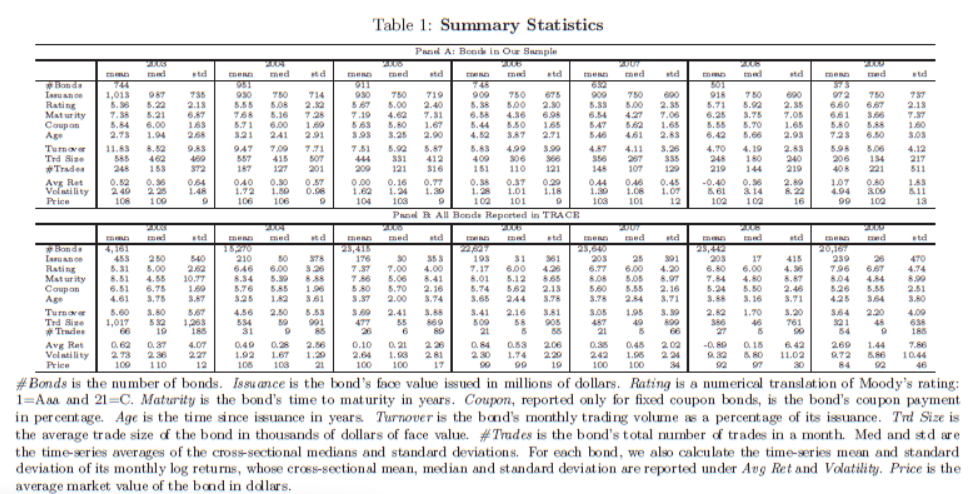
\includegraphics[width=0.75\textwidth]{\PathToAssets/table1_screenshot.jpg}
\end{figure}


\begin{table}[hbt!]
\centering
\textbf{\large Replicate Tables 1 in the Paper, For period 2003/04-2009/06: Panel A: Bonds in Our Sample, 2003-2009}
\resizebox{\textwidth}{!}{%
    \input{\PathToOutput table1_panelA.tex}
}
\label{table:table1_panelA}
\end{table}


\begin{table}[hbt!]
\centering
\textbf{\large Replicate Tables 1 in the Paper, For period 2003/04-2009/06: Panel B: All Bonds Reported in TRACE, 2003-2009}
\resizebox{\textwidth}{!}{%
    \input{\PathToOutput table1_panelB.tex}
}
\label{table:table1_panelB}
\end{table}


\begin{table}[hbt!]
\centering
\textbf{\large Update Table 1 in the Paper, For period 2009/06-Present: Panel A: Bonds in Our Sample, 2003-Present}
\resizebox{\textwidth}{!}{%
    \input{\PathToOutput table1_panelA_uptodate.tex}
}
\label{table:  table1_panelA_uptodate}
\end{table}


\begin{table}[hbt!]
\centering
\textbf{\large Update Table 1 in the Paper, For period 2009/06-Present: Panel B: All Bonds Reported in TRACE, 2003-Present}
\resizebox{\textwidth}{!}{%
    \input{\PathToOutput table1_panelB_uptodate.tex}
}
\label{table:  table1_panelB_uptodate}
\end{table}



\subsection{Table 2 Measure of Illiquidity $ \gamma = -\text{Cov}(p_t - p_{t-1}, p_{t+1} - p_t) $ }


Table 2 summarizes the illiquidity measure $\gamma$ for the bonds in our sample. \textbf{Table 2 Measure of Illiquidity} contains 3 panels: illiquidity of individual bonds, of bond portfolios and implied by quoted bid-ask spreads.

\begin{itemize}
    \item \textbf{Panel A Individual Bonds} (The mean and average monthly illiquidity per bond per year)
    \begin{itemize}
        \item Using trade-by-trade data
        \item Using daily data
        \begin{itemize}
            \item Using our cleaned original data
            \item Using our cleaned MMN corrected data
        \end{itemize}
    \end{itemize}
    
    \item \textbf{Panel B Bond Portfolio}
    \begin{itemize}
        \item \textbf{Equal-weighted:} Consider a daily portfolio composed of all bonds, with equally weighted bond returns used to calculate monthly illiquidity and median illiquidity per year
        \item \textbf{Issuance-weighted:} Consider a daily portfolio composed of all bonds, with issuance weighted bond returns used to calculate monthly illiquidity and median illiquidity per year
    \end{itemize}
    
    \item \textbf{Panel C Implied by quoted bid-ask spread}
    \begin{itemize}
        \item Mean and median monthly bond bid-ask spread per year
    \end{itemize}
\end{itemize}


\begin{figure}[hbt!]
\centering
\textbf{\large Original Table 2 in the paper}
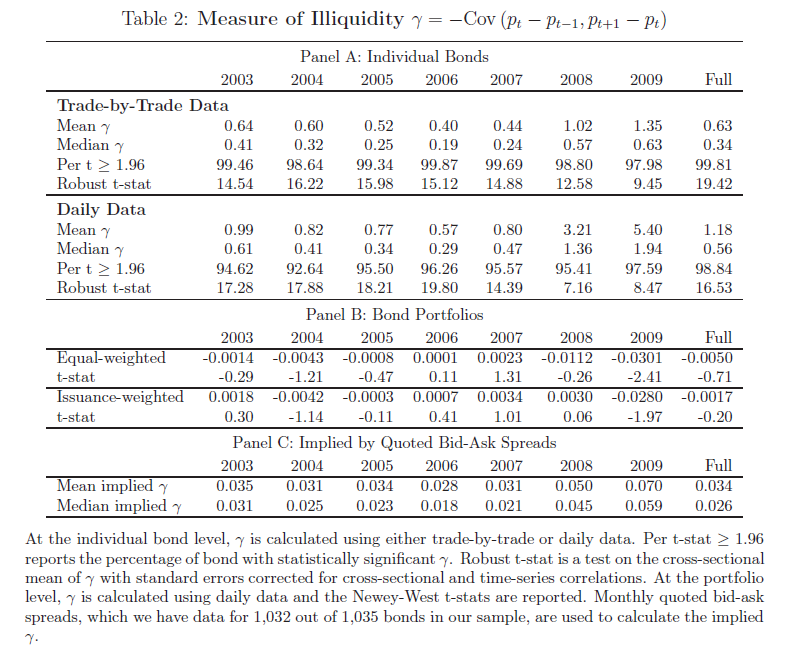
\includegraphics[width=0.75\textwidth]{\PathToAssets/table2_screenshot.jpg}
\end{figure}

\textbf{\large Table 2 Panel A Daily Data}

During the period covered by the paper, spanning from 2003 to 2009, the illiquidity metric $\gamma$ exhibited a mean value of 3.12 and a median of 0.07, with a substantial t-statistic of 17.06 using daily data. This compares to an average of 1.18 and a median of 0.56 observed in the paper. Our analysis successfully mirrored the initial decline followed by a subsequent rise in trends as documented in the original study. While other illiquidity metrics maintained a deviation within 40\% when compared to the original findings, the illiquidity we recorded for 2008--2009 were significantly higher -- by a factor of 3 to 4 times -- potentially influenced by approximately six bonds exhibiting $\gamma$ values exceeding 2000. The original study, however, did not specify an approach for managing outliers, leaving us uncertain whether these variations arise from outlier effects or inherent differences in data. In addition, our percentage of illiquidity significant at 95\% level is much lower than what the paper has, suggesting that the authors might have handled outliers somewhat differently to maintain higher significance. 6 out of 8 robust t-stats are significant at 95\% level in our analysis, with the overall robust t-stat = 17.6, close to the 16.53 in the paper, indicating the overall significance of the data.


\textbf{\large Table 2 Panel B Bond Portfolio}

For Panel B, we constructed two sets of daily bond portfolios from the same cross-section of bonds and for the same sample period, one being equally weighted and the other being weighted by issuance. After obtaining the daily portfolio returns (using $\Delta \log$ bond price) and lag returns (using $\Delta \log$ bond price lag), we calculated the monthly illiquidity through negative covariance of the returns and lag returns and then found the median per year for two sets of portfolios. The paper suggests that this measure implies that the transitory component extracted by the $\gamma$ measure is idiosyncratic in nature and gets diversified away at the portfolio level, but a suspected systematic component is present when this aggregate illiquidity measure comoves strongly with the aggregate market condition at the time. Similar to the paper, our peak in illiquidity appeared in $\sim$2006--2007, and most of the portfolio illiquidity measures were not statistically significant. All measures replicate the paper within a tolerance of $\pm$0.05 (equal-weighted), $\pm$0.07 (issuance-weighted).


\textbf{\large Table 2 Panel C Bid-Ask Spread}

In Panel C, we computed the monthly average and median bid-ask spreads for each year, using these as proxies for implied illiquidity. The methodology involved utilizing the monthly bond return data available on WRDS to calculate the t-spreads, whereas the original authors derived their data from daily figures, potentially accounting for some differences in results. Despite these differences, by applying a factor of 5 to our findings, we were able to align our results with the original study's observed pattern of initial decline followed by an increase in illiquidity, with a tolerance level below 40\%. It is noteworthy that the mean bid-ask spread for 2005 exhibited a slight increase in our table, although the median remained lower than that of the preceding year. This discrepancy underscores the influence of outliers on the mean and indicates a positive skew in the data.



\doublespacing
\begin{table}[hbt!]
\centering
\textbf{\large Replicate Table 2 in the Paper, For period 2003/04-2009/06: Panel A: Individual Bonds, Trade-by-Trade Data, 2003-2009}
\input{\PathToOutput table2_panelA_trade_by_trade_paper.tex}
\label{table:table2_panelA_trade_by_trade_paper}
\end{table}

\begin{table}[hbt!]
\centering
\textbf{\large Replicate Table 2 in the Paper, For period 2003/04-2009/06: Panel A: Individual Bonds, Daily Data, 2003-2009}
\input{\PathToOutput table2_panelA_daily_paper.tex}
\label{table:table2_panelA_daily_paper}
\end{table}

\begin{table}[hbt!]
\centering
\textbf{\large Replicate Table 2 in the Paper, For period 2003/04-2009/06: Panel B: Bond Portfolios, 2003-2009}
\input{\PathToOutput table2_panelB_paper.tex}
\label{table:table2_panelB_paper}
\end{table}

\begin{table}[hbt!]
\centering
\textbf{\large Replicate Table 2 in the Paper, For period 2003/04-2009/06: Panel C: Implied by Quoted Bid-Ask Spreads, 2003-2009}
\input{\PathToOutput table2_panelC_paper.tex}
\label{table:table2_panelC_paper}
\end{table}



\begin{table}[hbt!]
\centering
\textbf{\large Update Table 2 in the Paper, For period 2003/04-Present: Panel A: Individual Bonds, Trade-by-Trade Datas, 2003-Present}
\resizebox{\textwidth}{!}{%
    \input{\PathToOutput table2_panelA_trade_by_trade_new.tex}
}
\label{table:table2_panelA_trade_by_trade_new}
\end{table}

\begin{table}[hbt!]
\centering
\textbf{\large Update Table 2 in the Paper, For period 2003/04-Present: Panel A: Individual Bonds, Daily Data, 2003-Present}
\resizebox{\textwidth}{!}{%
    \input{\PathToOutput table2_panelA_daily_new.tex}
}
\label{table:table2_panelA_daily_new}
\end{table}


\begin{table}[hbt!]
\centering
\textbf{\large Update Table 2 in the Paper, For period 2003/04-Present: Panel B: Bond Portfolios, 2003-Present}
\resizebox{\textwidth}{!}{%
    \input{\PathToOutput table2_panelB_new.tex}
}
\label{table:table2_panelB_new}
\end{table}


\begin{table}[hbt!]
\centering
\textbf{\large Update Table 2 in the Paper, For period 2003/04-Present: Panel C: Implied by Quoted Bid-Ask Spreads, 2003-Present}
\resizebox{\textwidth}{!}{%
    \input{\PathToOutput table2_panelC_new.tex}
}
\label{table:table2_panelC_new}
\end{table}



\begin{table}[hbt!]
\centering
\textbf{\large Table 2 Panel A Daily Data using MMN-Corrected Bond Data}
\textbf{\large Panel A: Individual Bonds, MMN-Corrected Bond Data, 2003-2009}
\input{\PathToOutput table2_daily_mmn_paper.tex}
\label{table:table2_daily_mmn_paper}
\end{table}


\begin{table}[hbt!]
\centering
\textbf{\large Individual Bonds, MMN-Corrected Bond Data, 2003-Present}
\resizebox{\textwidth}{!}{%
    \input{\PathToOutput table2_daily_mmn_new.tex}
}
\label{table:table2_daily_mmn_new}
\end{table}


\subsection{Monthly Bond Illiquidity Summary Statistics}

By integrating the summary statistics and graphical representations of monthly bond illiquidity, we gain insight into the pronounced fluctuations in illiquidity, particularly during the 2008 sub-prime crisis. The summary statistics offer a comprehensive view of the annual distribution of illiquidity, highlighting extreme peaks of over 5000 in 2008 and over 8000 in 2009. In contrast, the third quartile remained between 1 and 2, indicating the presence of significant outliers, likely driven by a few bonds with gamma values surpassing 2000. Despite these spikes, the median values of 0.23 and 0.33 in 2008 and 2009, respectively, were considerably lower than the mean values of 13.27 and 17.98, suggesting a generally higher liquidity level during these years. Extending the analysis to 2023 revealed notable surges in illiquidity in 2018 and 2020.

The scatter plots visualize monthly illiquidity for individual bonds, with the red and purple lines delineating the mean and median annual illiquidity, respectively. These plots uncover a declining trend in monthly bond illiquidity, succeeded by a rising trend leading up to 2009, marked by exceptionally high illiquidity instances reaching up to 8000. Closer examination of the subsequent plot, which zooms in on the data, shows most values clustering in the 0-200 range. Notably, the mean illiquidity consistently exceeds the median during 2007-2009, reflecting a positive skew in the data attributed to outliers. The period post-2010 is characterized by more stable fluctuations, possibly due to a decrease in bond numbers following phase III. The MMN-corrected dataset presents a more uniform distribution, reducing outlier impact while preserving the identified trends.


\begin{table}[hbt!]
\centering
\textbf{\large Monthly Bond Illiquidity Summary Statistics Using Daily Data, 2003-2009}
\input{\PathToOutput illiq_summary_paper.tex}
\label{table:illiq_summary_paper}
\end{table}




\begin{table}[hbt!]
\centering
\textbf{\large Monthly Bond Illiquidity Summary Statistics Using Daily Data, 2003-Present}
\resizebox{\textwidth}{!}{%
    \input{\PathToOutput  illiq_summary_new.tex}
}
\label{table: illiq_summary_new}
\end{table}




\begin{table}[hbt!]
\centering
\textbf{\large Monthly Bond Illiquidity Summary Statistics Using MMN-Corrected Bond Data, 2003-2009}
\input{\PathToOutput illiq_daily_summary_mmn_paper.tex}
\label{table:illiq_daily_summary_mmn_paper}
\end{table}


\begin{table}[hbt!]
\centering
\textbf{\large Monthly Bond Illiquidity Summary Statistics Using MMN-Corrected Bond Data, 2003-Present}
\resizebox{\textwidth}{!}{%
    \input{\PathToOutput illiq_daily_summary_mmn_new.tex}
}
\label{table: illiq_daily_summary_mmn_new}
\end{table}


\section{Visualizations}

\begin{figure}[hbt!]
\centering
\textbf{\large Monthly Illiquidity Per Bond and Average Illiquidity By Year (See combined observations in the previous section)}
\caption{Illiquidity by Year with Mean Illiquidity, 2003-2009}
  \centering
  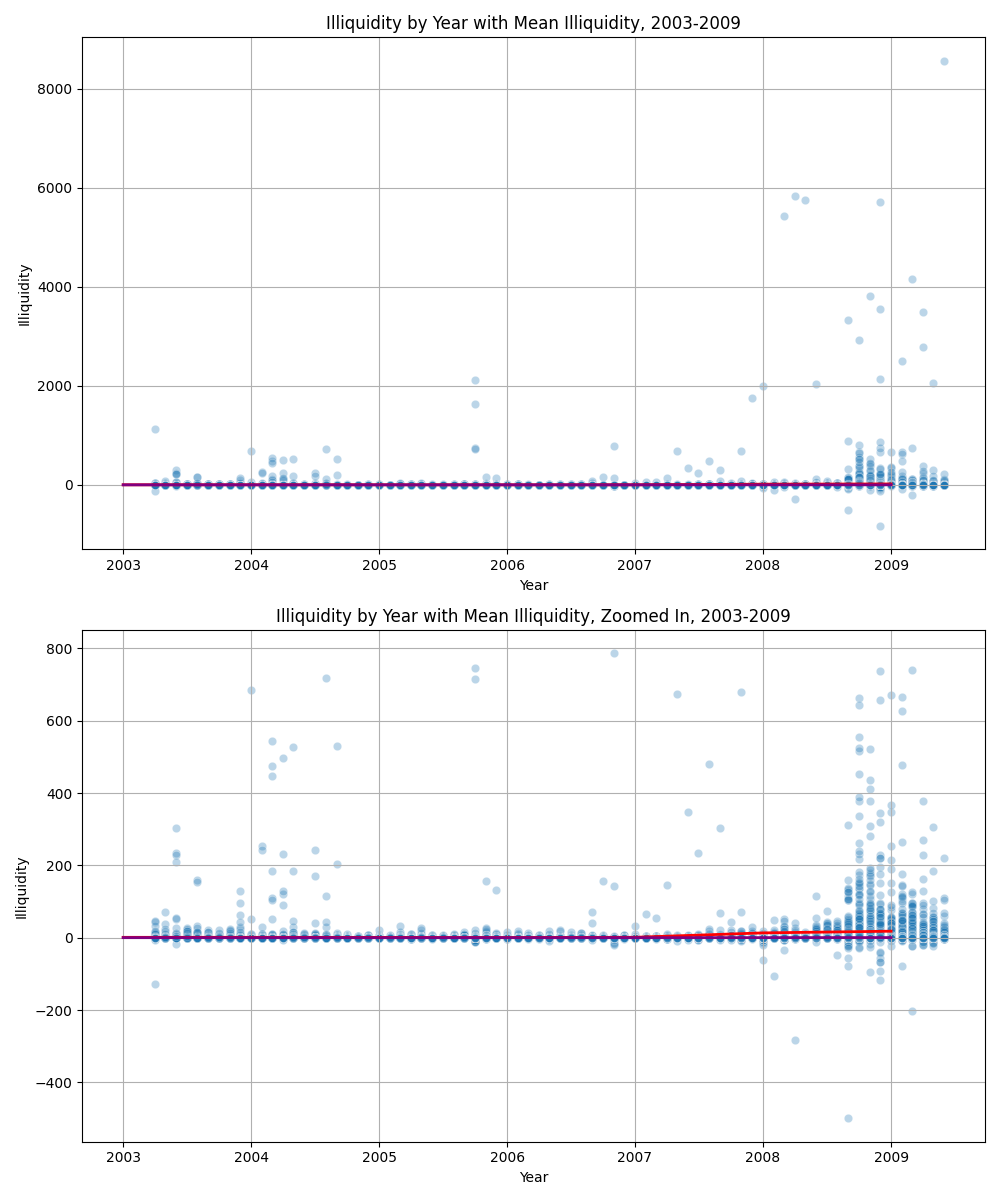
\includegraphics[width=0.75\linewidth]{\PathToOutput/illiq_plot_2003-2009.png}
  % \caption{Average returns}

\label{fig:illiq_plot_2003-2009}
\end{figure}


\begin{figure}[hbt!]
\centering
\caption{Illiquidity by Year with Mean Illiquidity, 2003-Present}
  \centering
  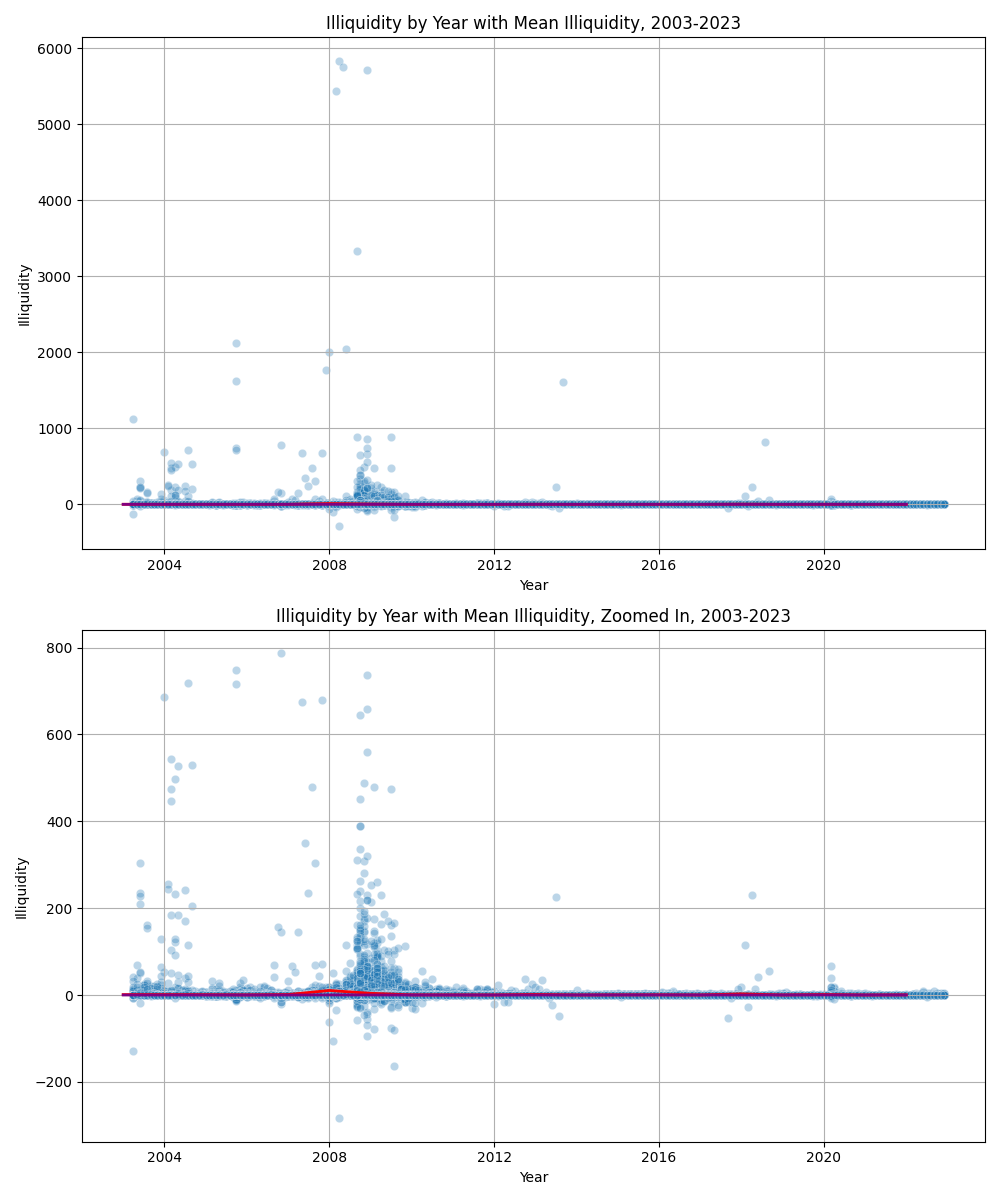
\includegraphics[width=0.75\linewidth]{\PathToOutput/illiq_plot_2003-2023.png}
  % \caption{Average returns}

\label{fig:illiq_plot_2003-2023}
\end{figure}



\begin{figure}[hbt!]
\centering
\textbf{\large Monthly Illiquidity Per Bond and Average Illiquidity By Year Using MMN-Corrected Data}
\caption{Illiquidity by Year with Mean Illiquidity Using MMN-Corrected Data, 2003-2009}
  \centering
  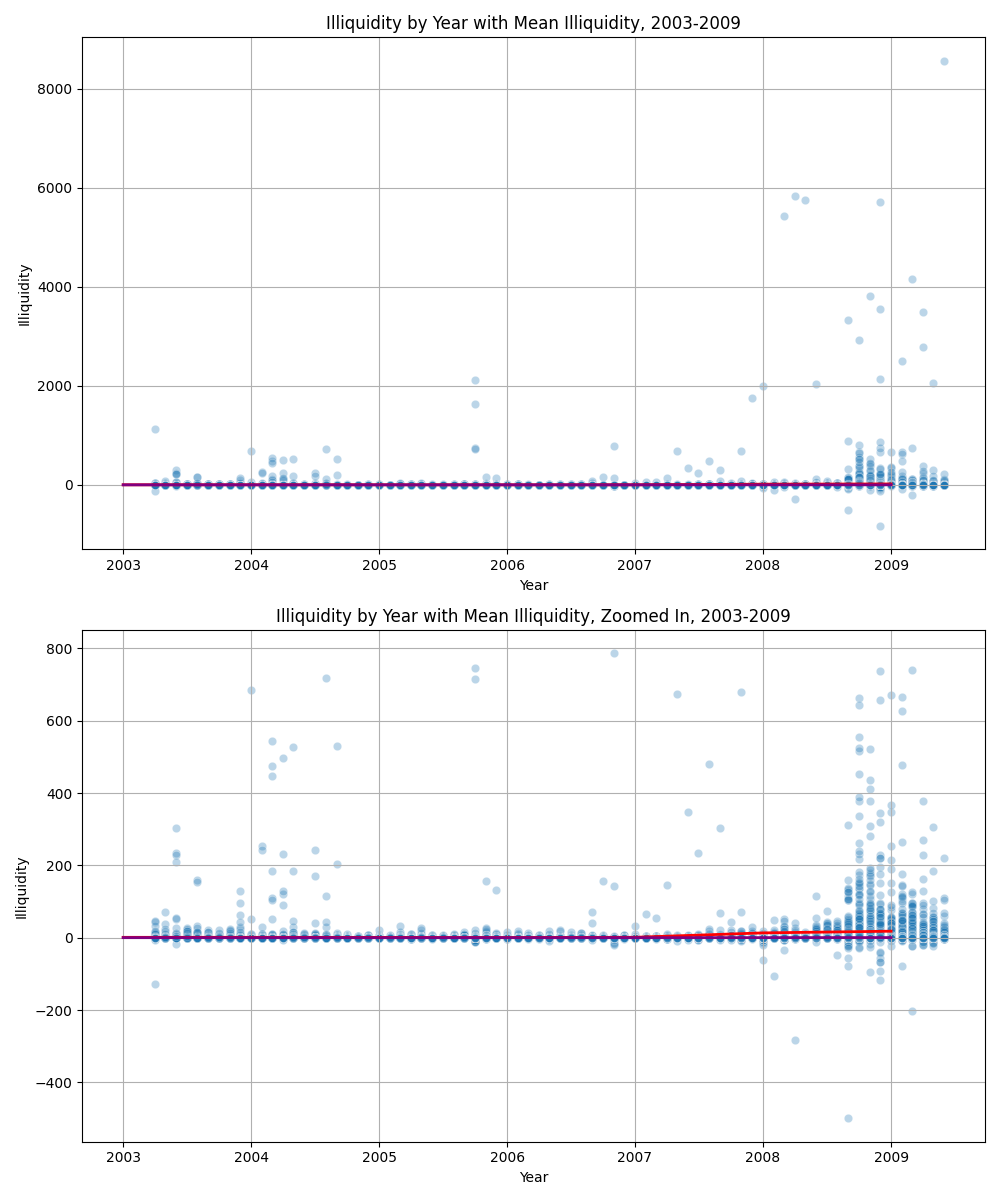
\includegraphics[width=0.75\linewidth]{\PathToOutput/illiq_plot_2003-2009.png}
  % \caption{Average returns}

\label{fig:illiq_plot_2003-2009}
\end{figure}


\begin{figure}[hbt!]
\centering
\caption{Illiquidity by Year with Mean Illiquidity Using MMN-Corrected Data, 2003-Present}
  \centering
  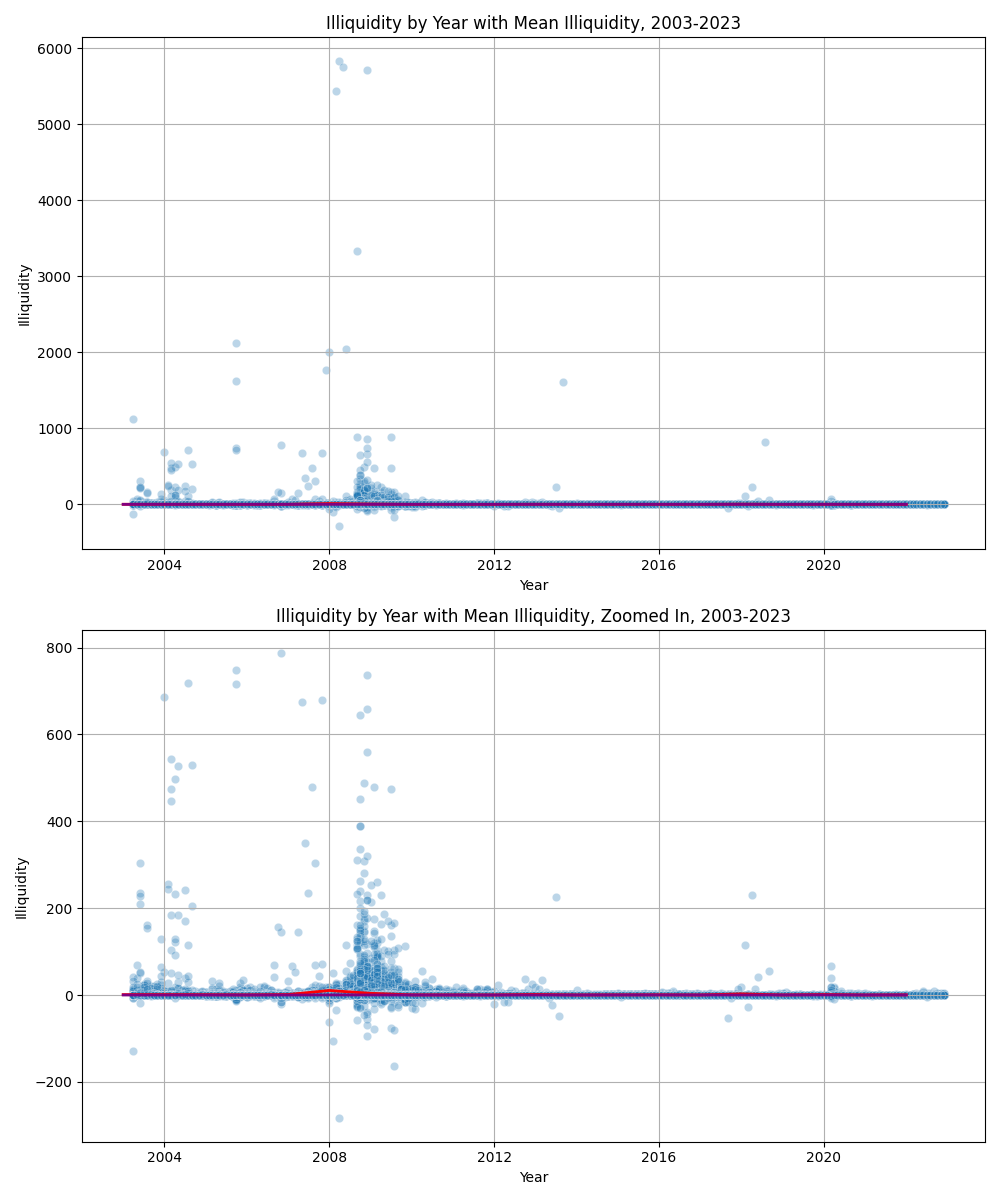
\includegraphics[width=0.75\linewidth]{\PathToOutput/illiq_plot_2003-2023.png}
  % \caption{Average returns}

\label{fig:illiq_plot_2003-2023}
\end{figure}


\end{document}